\chapter{Summary of Future Work}

\section{Automate generating process for a system of higher-order ODEs}
Chapter 4 discusses how to automate generating process for a single higher-order linear ODE. A system of higher-order ODE is multiple higher-order ODEs in one system. Generally, we can transform each individual higher-order ODE into a system of first-order ODE. This result in multiple system of first-order ODEs. We have to combine them into one system. The difficulty may come from how to represent a non-linear ODE. If we have a system of higher-order linear ODE, we can do steps in Chapter 4 to transform a higher-order linear ODE into a system of first-order ODE. However, more research is still needed to tackle a non-linear ODE.

\section{Generate an ODE Solver Object that Returns Solution on Demand}
Drasil has options for generating a runnable program or standalone libraries. However, all the current ODE-related case studies generate a runnable program. The requirement specify the output to be calculated. Chapter 3 analyzed each selected external library and provides two additional specifications. One of them output the ODE as a function that can return the value of the dependent variable for any value of the independent variable. If other outside programs want to utilize Drasil generated code, this requirement can be the start point.

% More research still needed to  

% For example, the Python Scipy library has an option to return a generic interface class that stores all necessary ODE information. C\# OSLO has an option for returning endless points. Those points are close to a mathematical definition of a spline. 

% Those two options provided by external libraries can be used for generating an ODE object that can return the value of the dependent variable for any value of the independent variable. Eventually, other outside programs can utilize Drasil generated ODE solvers.

\section{Display ODEs in Various Forms}
In Figure~\ref{fig_multienv}, we displayed the ODE in two different forms. In future, we want to display ODE in other forms. For example, in mathematical expression, sometimes we move all the terms to the left-hand side and leave the right-hand side to 0.
\begin{figure}[ht]
\centering	
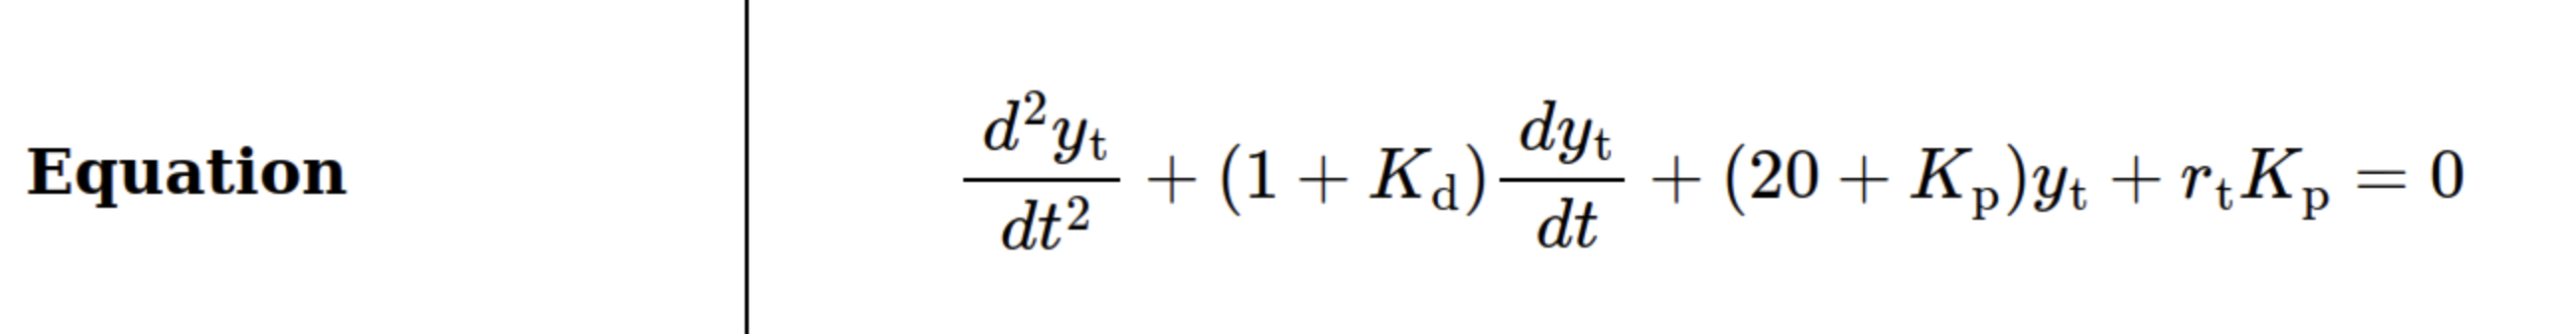
\includegraphics[width=1\textwidth]{figures/ODEVariousForm.png}
\caption{Options of Displaying an ODE}
\label{fig_odevariousform}
\end{figure}
This is just one example of the variability of displaying ODEs. More research still needed to allow Drasil displays ODEs in various forms.

\section{Allow Adaptive Steps}
While we were solving the ODE as an IVP numerically, we set the step size to fixed step size. In reality, the step size can be adaptive rather than fixed. We found some algorithms use a fixed step size for calculating numerical solutions, and others use an adaptive step size. We add the step size with the current time value to calculate the next value of dependent variables. A fixed step size means the step size is the same in each iteration. An adaptive step size means the step size is not always the same and could change based on other factors. In Table~\ref{tab_algacm}, the ACM library divides algorithms into one group that uses a fixed step and others that uses an adaptive step. This discovery can further influence the design choice of solving ODE numerically in the Drasil framework. Currently, Drasil treats all step sizes as a fixed value, and it would be ideal to allow the step size to be either fixed or adaptive in future.

\section{Handle Dependency}
Once the Drasil framework generates code, the generated code relies on external libraries to calculate an ODE. In the current setting, the Drasil framework keeps copies of external libraries in the repository. In the long run, this is not practical because of the amount of space external libraries occupy. Moreover, external libraries are not currently shared across case studies, and each case study will have its own copy of external libraries. The current research has uncovered that the current way of handling dependencies in the Drasil framework is problematic. In the future, the team would like to find a better way to handle dependencies. We used a temporary solution, symbolic links, to share external libraries without duplications. By creating a symbolic link file, external libraries become sharable. In the future, the team will conduct further studies to tackle this problem.

\section{Define ODE Solver in Drasil}
Our ultimate goal is to write the ODE solver in Drasil language. Currently, the ODE solver is four selected external libraries. They help us to produce a numerical solution. In future, we want to remove all external libraries and design Drasil's ODE solvers to solve ODEs. 
